\documentclass[11pt,a4paper]{article}
\usepackage[T1]{fontenc}
\usepackage{lmodern}
\usepackage[margin=23mm]{geometry}
\usepackage{graphicx,array,longtable,booktabs,caption,pdflscape,tikz}
\usetikzlibrary{positioning,arrows.meta}
\usepackage[hidelinks]{hyperref}
\hypersetup{pdftitle={Sprint I Security Incident Detection and Response Management System},pdfauthor={Christophe ElChabab}}
\setlength{\parindent}{0pt}
\setlength{\parskip}{6pt}
\setlength{\emergencystretch}{3em}
\captionsetup{font=small,labelfont=bf}
\newcommand{\pending}[1]{\par\textbf{Pending team input:} #1\par}
\newcommand{\evidencefigure}[2]{%
\clearpage\begin{figure}[p]\centering
\IfFileExists{evidence/#1}{\includegraphics[width=\linewidth,height=0.84\textheight,keepaspectratio]{evidence/#1}}{\includegraphics[width=\linewidth,height=0.84\textheight,keepaspectratio]{../../Christophe-ElChabab-Screenshots/#1}}
\caption{#2}
\end{figure}\clearpage}
\begin{document}
\begin{titlepage}
\centering
{\Large American University of Beirut\par}
{\large EECE 435L\par}
\vspace{15mm}
{\LARGE\bfseries Security Incident Detection and Response Management System\par}
\vspace{8mm}
{\Large Sprint I Report\par}
\vspace{12mm}
Christophe ElChabab\par Joey Saade\par Karl Khouri\par
\vspace{10mm}
Date of submission: to be confirmed\par
\vfill
\textbf{Draft for team completion}\par
Christophe's service explanations and actual local execution evidence are included. Teammate implementation sections, final GitHub evidence and CREATES feedback remain to be completed. This is not the final common submission.\par
\end{titlepage}
\tableofcontents
\clearpage
\section{Introduction (Christophe ElChabab)}
The system organizes security incident reporting, investigation and response. It links affected assets to vulnerabilities and incidents, maintains threat indicators, records security activity, notifies users and generates reports.
Sprint I implements backend APIs and persistent storage rather than a graphical interface. The goals are validated input, authenticated role-based access, traceable investigation workflows and API integration across the nine services.
\section{System Architecture (Christophe ElChabab)}
Nine FastAPI processes share a local SQLite database for identity and foreign-key relationships. Services expose owner-prefixed routes. Audit and notification events are delivered over HTTP using service credentials; reports retrieve data through service APIs.
\begin{figure}[htbp]\centering
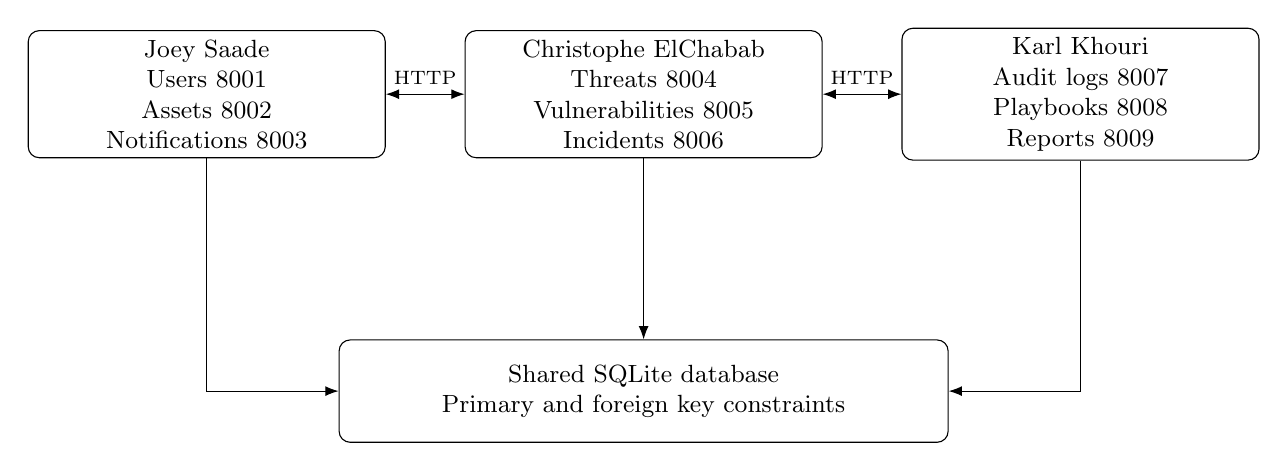
\begin{tikzpicture}[box/.style={draw,rounded corners,align=center,font=\small,text width=43mm,minimum height=13mm},>=Latex]
\node[box] (j) {Joey Saade\\Users 8001\\Assets 8002\\Notifications 8003};
\node[box,right=10mm of j] (c) {Christophe ElChabab\\Threats 8004\\Vulnerabilities 8005\\Incidents 8006};
\node[box,right=10mm of c] (k) {Karl Khouri\\Audit logs 8007\\Playbooks 8008\\Reports 8009};
\node[box,below=23mm of c,text width=75mm] (d) {Shared SQLite database\\Primary and foreign key constraints};
\draw[<->] (j) -- node[above,font=\scriptsize]{HTTP} (c);
\draw[<->] (c) -- node[above,font=\scriptsize]{HTTP} (k);
\draw[->] (j.south) |- (d.west);
\draw[->] (c.south) -- (d.north);
\draw[->] (k.south) |- (d.east);
\end{tikzpicture}
\caption{Christophe ElChabab - System architecture - Shows service ownership, ports, HTTP integration and shared storage.}
\end{figure}
The arrows describe the implemented data flow, not independent student authorship of shared code. Users authenticate through Joey's service. Christophe's mutations queue events transactionally; delivery sends them to audit logging and notifications. Karl's reports call the relevant list APIs with the requesting user's token.
\section{Implementation Details}
\subsection{Users Assets and Notifications (Joey Saade)}
\pending{Joey supplies his reviewed implementation explanations, request/response formats, database interactions and actual execution evidence.}
\subsection{Threats Vulnerabilities and Incidents (Christophe ElChabab)}
The Threat Intelligence, Vulnerability Management and Incident Management services run as separate FastAPI processes on ports 8004, 8005 and 8006. Their 18 business endpoints use the prefix \texttt{/api/Christophe-ElChabab}. The source files are \texttt{christophe/threats.py}, \texttt{christophe/vulnerabilities.py}, \texttt{christophe/incidents.py} and \texttt{christophe/schema.sql}.

Joey Saade's Users service authenticates users and issues bearer tokens. Each request checks the authenticated account and its current role. Users and Assets are shared database entities; Christophe's services reference them instead of creating separate copies. Mutations queue audit and notification events in the same database transaction. After commit, delivery calls Karl Khouri's Audit service and Joey Saade's Notifications service over HTTP. Failed deliveries remain queued for retry. Karl's Reports service reads the list APIs over HTTP.

\subsection{Threat Intelligence (Christophe ElChabab)}

Administrators create indicators with a type, value, description, severity and source. Reads return IDs and UTC creation/update timestamps alongside those fields. List and search return JSON arrays; detail returns one object. Search accepts type, value, severity and source, combining supplied conditions with AND. Updates accept description, severity and source. Deletion returns a confirmation message.

IP addresses, domain syntax and hexadecimal file hashes are validated according to their indicator type. Normalization precedes the unique type/value check, so repeated indicators return 409. The captured duplicate, invalid address/hash/domain and missing-field requests demonstrate rejection. Only administrators can mutate threats; analysts and auditors can read/search. The professor confirmed that auditors may use GET /threats/search.

Two synthetic indicators were used in the real local execution: a Domain indicator and IP indicator 198.51.100.42. They are test inputs, not assertions of real malicious activity. The domain was initially High and then updated to Critical with source Investigation; the IP was Critical with source SOC. These classifications exercise the stored severity/source fields and filtering. Before Cleanup, the database and threat report both contained two Critical indicators. Successful deletion and the subsequent 404 for the domain are captured separately.

\subsection{Vulnerability Management (Christophe ElChabab)}

Administrators create vulnerabilities with title, description, CVE ID, CVSS score, explicit severity, affected asset ID and source. Creation returns the stored object with status Open. Reads and searches return the stored fields and server timestamps. Search supports CVE ID, severity, asset ID and status, combining supplied filters with AND.

CVSS must be a finite number from 0 to 10; booleans are not valid scores or IDs. CVE validation checks the CVE-YYYY-NNNN syntax with at least four final digits; it does not verify a vulnerability against an external registry. The affected asset must exist. Captures demonstrate malformed CVEs, invalid CVSS and an unknown asset returning 422. Administrators and analysts can update permitted fields; auditors cannot update, and only administrators can delete.

The required remediation sequence is Open -> Under Investigation -> In Progress -> Resolved -> Closed. Skipping a state returns 409. The server sets the resolution timestamp at Resolved and retains it at Closed. Every transition is captured.

The first test record starts at CVSS 8.1/High, then is updated to 9.1/Critical and reaches Closed. The second remains 5.0/Medium/Open. The Critical/High/Medium values are explicit test classifications; they demonstrate priority differences rather than verified production risk. Before Cleanup, the report and database agree on one Critical Closed record and one Medium Open record, with average CVSS (9.1 + 5.0) / 2 = 7.05.

\subsection{Incident Management (Christophe ElChabab)}

Administrators and employees can report an incident with title, description, category, severity, reporter ID and asset ID. The reporter and asset must exist. An employee cannot submit under another user's identity. Creation returns a new Open incident; assignment requires an active Security Analyst and administrator permission.

The professor confirmed that GET /incidents is available to all four roles. Administrators and auditors see all incidents, analysts see only their assignments, and employees see only their submissions. These restrictions derive from authenticated identity. Forged reporter, assignee or role query parameters do not broaden access. The screenshots show employee 4 seeing records 1 and 2, while the other employee's record 3 is excluded; analyst 2 sees only assigned record 1.

The sequence is Open -> Under Investigation -> Mitigated -> Resolved -> Closed. Only administrators or the assigned analyst may change status. Skips are rejected with 409. The captured workflow includes all transitions and retention of the resolution timestamp.

Authorized staff add a nonblank investigation note. The server records the authenticated author, incident ID and creation timestamp, rather than accepting a forged author from the request. The stored note is linked to incident 1 and analyst 2 and appears in the retrieved incident. No incident DELETE endpoint is added because the handout does not request one.

The three test incidents use High, Critical and Medium severity. High represents the primary suspicious-message investigation, Critical the higher-priority comparison scenario, and Medium the other reporter's lower-priority scenario. These are test classifications, not evidence that an actual compromise occurred. The different reporters and severities exercise priority storage and identity-based access. At the end of the captured workflow, incident 1 is Closed/High and assigned to analyst 2; incident 2 is Open/Critical and incident 3 is Open/Medium.

\subsection{Audit Logging Playbooks and Reports (Karl Khouri)}
\pending{Karl supplies his reviewed implementation explanations and actual execution evidence. Christophe's integration screenshots do not replace Karl's endpoint evidence.}
\section{Database Design (Christophe ElChabab)}
The four owned tables use integer primary keys. Threats enforce uniqueness on (type, value). Vulnerabilities reference assets.id. Incidents reference users.id through reporter\_id and assigned\_to, and assets.id through asset\_id. Investigation notes reference incidents.id and users.id through analyst\_id. One asset can have many vulnerabilities and incidents; one reporter can submit many incidents; one analyst can have many assignments/notes; one incident can contain many notes.

User/asset references restrict deletion while still referenced. Note rows specify ON DELETE CASCADE for their incident foreign key. Severity, CVSS and lifecycle CHECK constraints supplement API validation. Resolution dates are nullable until resolution. The schema captures below display the actual table definitions, including primary and foreign keys. The record captures were taken before the authorized threat/vulnerability Cleanup requests.

\begin{figure}[htbp]\centering
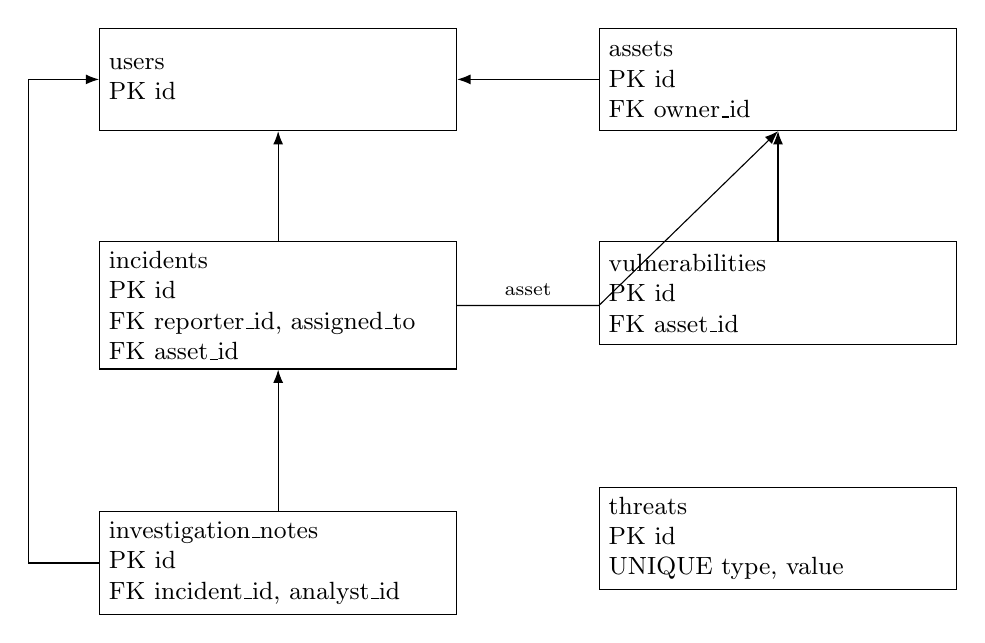
\begin{tikzpicture}[box/.style={draw,align=left,font=\small,text width=43mm,minimum height=13mm},>=Latex]
\node[box] (u) {users\\PK id};
\node[box,right=18mm of u] (a) {assets\\PK id\\FK owner\_id};
\node[box,below=14mm of u] (i) {incidents\\PK id\\FK reporter\_id, assigned\_to\\FK asset\_id};
\node[box,below=14mm of a] (v) {vulnerabilities\\PK id\\FK asset\_id};
\node[box,below=18mm of i] (n) {investigation\_notes\\PK id\\FK incident\_id, analyst\_id};
\node[box,below=18mm of v] (t) {threats\\PK id\\UNIQUE type, value};
\draw[->] (a.west) -- (u.east);
\draw[->] (i.north) -- (u.south);
\draw[->] (i.east) -- node[above,font=\scriptsize]{asset} (v.west |- i.east) -- (a.south);
\draw[->] (v.north) -- (a.south);
\draw[->] (n.north) -- (i.south);
\draw[->] (n.west) -- ++(-9mm,0) |- (u.west);
\end{tikzpicture}
\caption{Christophe ElChabab - Owned service schema - Arrows point from foreign-key tables to referenced tables. Users and Assets belong to Joey's services.}
\end{figure}
The appendix contains actual SQL table definitions and rows with column labels for all four Christophe tables.
\pending{Merge the remaining team schema (notifications, audit logs, playbooks, response actions and supporting history/outbox tables), field explanations and teammate database evidence into the common schema documentation.}
\section{Error Handling and Validation (Christophe ElChabab)}
The real API evidence covers successful calls, invalid formats/ranges/references, duplicates, unknown IDs, missing authentication, forbidden mutations, incident ownership and assignment, spoofed query scope, lifecycle skips and blank notes. The captured integration calls show the incident-assignment notification, threat audit events, assignment audit event and denied-access audit records.

The pre-Cleanup reports match the captured database: two threats, two vulnerabilities and three incidents. The summary reports complete=true and an empty unavailable list. Integration routes retain Joey Saade's and Karl Khouri's prefixes because those services belong to them; these captures demonstrate Christophe's integration, not ownership of their implementations.

Screenshots were captured by Christophe from his running local environment. Codex inspected and organized the originals without changing their image bytes. The screenshot set below contains 84 API/integration captures and eight database captures. Cleanup shows four successful deletions and two expected 404 confirmations; the database record screenshots document the earlier populated state.

\section{API Documentation (Christophe ElChabab)}
All suffixes below follow \texttt{/api/Christophe-ElChabab}. Administrator, Analyst and Auditor mean the Security Administrator, Security Analyst and Security Auditor roles. Employee means Regular Employee.

\begin{small}
\begin{longtable}{p{0.09\linewidth}p{0.22\linewidth}p{0.32\linewidth}p{0.25\linewidth}}
\toprule
Method & Suffix & Function & Authorized roles \\
POST & /threats & Create indicator & Administrator \\
GET & /threats & List indicators & Administrator, Analyst, Auditor \\
GET & /threats/\{id\} & Retrieve indicator & Administrator, Analyst, Auditor \\
GET & /threats/search & Filter type, value, severity, source & Administrator, Analyst, Auditor \\
PUT & /threats/\{id\} & Update description, severity, source & Administrator \\
DELETE & /threats/\{id\} & Delete indicator & Administrator \\
POST & /vulnerabilities & Create vulnerability & Administrator \\
GET & /vulnerabilities & List vulnerabilities & Administrator, Analyst, Auditor \\
GET & /vulnerabilities/\{id\} & Retrieve vulnerability & Administrator, Analyst, Auditor \\
GET & /vulnerabilities/search & Filter CVE, severity, asset, status & Administrator, Analyst, Auditor \\
PUT & /vulnerabilities/\{id\} & Update vulnerability and remediation state & Administrator, Analyst \\
DELETE & /vulnerabilities/\{id\} & Delete vulnerability & Administrator \\
POST & /incidents & Report incident & Administrator, Employee \\
GET & /incidents & List within authenticated scope & All four roles with restrictions \\
GET & /incidents/\{id\} & Retrieve incident & Administrator, Auditor, assigned Analyst, original Employee \\
PUT & /incidents/\{id\}/assign & Assign analyst & Administrator \\
PUT & /incidents/\{id\}/status & Change lifecycle state & Administrator, assigned Analyst \\
POST & /incidents/\{id\}/notes & Add investigation note & Administrator, assigned Analyst \\
\bottomrule
\end{longtable}
\end{small}

Creation returns 201; successful reads, searches, updates and deletions return 200. Detail responses are objects, lists/searches return arrays, and deletions return a message. Unknown IDs return 404. Error responses contain status and message; validation responses can also contain field-specific errors. Missing authentication returns 401, insufficient permission returns 403, duplicates/invalid transitions return 409, and invalid input/references return 422. SQL values use bound parameters, and accepted filter fields are fixed server-side.

The importable request collection is \texttt{postman/christophe.collection.json}. The public environment template is \texttt{postman/christophe.environment.template.json}. Credentials must be supplied privately; local secrets and access tokens are not submission material.

Detailed real request and response examples appear in the captioned appendix. Import postman/christophe.collection.json with the credential-free environment template, then set private credentials locally. Do not publish access tokens or private environment files.
\pending{Merge Joey's and Karl's complete API references and Postman collections.}
\section{Authentication and Authorization (Christophe ElChabab)}
Joey's Users service issues signed bearer tokens. Protected calls verify the token and current account status, then apply role and object-level authorization. The four role names are Security Administrator, Security Analyst, Security Auditor and Regular Employee.
The professor confirmed auditor access to threat searching and identity-scoped incident lists. These permissions are included in the endpoint reference and real tests. A supplied role, reporter or assignee query parameter cannot replace authenticated identity.
The shared authentication appendix includes a successful administrator login and an incorrect-password request returning 401. Both use Joey's login route; Christophe captured them to demonstrate the authentication dependency. They are not additional Christophe APIs. Insufficient and correct permissions are demonstrated on Christophe's routes in the service evidence.
\section{GitHub and Version Control (Christophe ElChabab)}
Repository: \url{https://github.com/chrs-005/ChristopheElChabab-JoeySaade-KarlKhouri}.
The original Christophe three-service implementation is recorded in commit \texttt{537e769}. Subsequent commits must describe actual changes and preserve genuine author identity and dates.
\pending{After final commits are pushed, insert actual commit-history and per-member contribution screenshots with captions. Do not create fictitious history or attribute generated code to unaided manual authorship.}
\section{References (Christophe ElChabab)}
Requirements source: Final Project Fall 2026-2027-Sprint 1.docx, supplied by the instructor. Permission clarifications: the professor's answers supplied by Christophe on 19 October 2026 concerning auditor threat searching and identity-scoped incident lists. Implementation references: the owned source/schema files, docs/christophe-api.md and the importable Postman collection.

Codex generated implementation, tests, documentation and Postman artifacts, assisted with local execution and review, and prepared this report section. Christophe captured the execution screenshots. This disclosure does not represent AI-generated code as independent manual student authorship or replace the course requirement to understand, review, adapt and explain the implementation.

\subsection*{CREATES completion}
\pending{Record the team's genuine CREATES session, received feedback and changes made. All three members must meet the timing and attendance requirements. No meeting or feedback is claimed here.}
\clearpage
\appendix
\section{Actual Execution Evidence (Christophe ElChabab)}
Captures are retained unchanged. Schema and stored-record screenshots precede Cleanup; later successful deletions therefore do not contradict the earlier populated state. Each caption identifies the capturer, operation and purpose. Shared login and integration screenshots retain their real service owners' routes.
\begin{landscape}
\evidencefigure{01-Shared-Authentication/01-Christophe-ElChabab-POST-Administrator-Login-200.png}{Christophe ElChabab - Successful authentication - Joey Saade's login API returns an access token for a valid administrator.}
\evidencefigure{01-Shared-Authentication/02-Christophe-ElChabab-POST-Reject-Incorrect-Password-401.png}{Christophe ElChabab - Failed authentication - Joey Saade's login API rejects an incorrect password with HTTP 401.}
\evidencefigure{02-Threat-Intelligence/01-Christophe-ElChabab-POST-Create-Domain-Threat-201.png}{Christophe ElChabab - POST Create Domain Threat - Shows the submitted request and the newly created record returned with HTTP 201.}
\evidencefigure{02-Threat-Intelligence/02-Christophe-ElChabab-POST-Create-IP-Threat-201.png}{Christophe ElChabab - POST Create IP Threat - Shows the submitted request and the newly created record returned with HTTP 201.}
\evidencefigure{02-Threat-Intelligence/03-Christophe-ElChabab-POST-Reject-Duplicate-Domain-409.png}{Christophe ElChabab - POST Reject Duplicate Domain - Shows that a duplicate indicator or invalid lifecycle change is rejected with HTTP 409.}
\evidencefigure{02-Threat-Intelligence/04-Christophe-ElChabab-POST-Reject-Invalid-IP-422.png}{Christophe ElChabab - POST Reject Invalid IP - Shows that invalid input or a reference is rejected with HTTP 422.}
\evidencefigure{02-Threat-Intelligence/05-Christophe-ElChabab-POST-Reject-Invalid-Hash-422.png}{Christophe ElChabab - POST Reject Invalid Hash - Shows that invalid input or a reference is rejected with HTTP 422.}
\evidencefigure{02-Threat-Intelligence/06-Christophe-ElChabab-POST-Reject-Malformed-Domain-422.png}{Christophe ElChabab - POST Reject Malformed Domain - Shows that invalid input or a reference is rejected with HTTP 422.}
\evidencefigure{02-Threat-Intelligence/07-Christophe-ElChabab-POST-Reject-Missing-Fields-422.png}{Christophe ElChabab - POST Reject Missing Fields - Shows that invalid input or a reference is rejected with HTTP 422.}
\evidencefigure{02-Threat-Intelligence/08-Christophe-ElChabab-GET-Reject-Employee-Threat-Access-403.png}{Christophe ElChabab - GET Reject Employee Threat Access - Shows that the unauthorized operation is refused with HTTP 403.}
\evidencefigure{02-Threat-Intelligence/09-Christophe-ElChabab-GET-Reject-Missing-Authentication-401.png}{Christophe ElChabab - GET Reject Missing Authentication - Shows that the unauthenticated request is rejected with HTTP 401.}
\evidencefigure{02-Threat-Intelligence/10-Christophe-ElChabab-GET-List-Threats-as-Auditor-200.png}{Christophe ElChabab - GET List Threats as Auditor - Shows the named request and its successful HTTP 200 result.}
\evidencefigure{02-Threat-Intelligence/11-Christophe-ElChabab-GET-Get-Threat-as-Analyst-200.png}{Christophe ElChabab - GET Get Threat as Analyst - Shows the named request and its successful HTTP 200 result.}
\evidencefigure{02-Threat-Intelligence/12-Christophe-ElChabab-GET-Reject-Unknown-Threat-ID-404.png}{Christophe ElChabab - GET Reject Unknown Threat ID - Shows that an unknown record returns HTTP 404.}
\evidencefigure{02-Threat-Intelligence/13-Christophe-ElChabab-GET-Search-Threats-by-Type-200.png}{Christophe ElChabab - GET Search Threats by Type - Shows the named request and its successful HTTP 200 result.}
\evidencefigure{02-Threat-Intelligence/14-Christophe-ElChabab-GET-Search-Threats-as-Auditor-200.png}{Christophe ElChabab - GET Search Threats as Auditor - Shows the named request and its successful HTTP 200 result.}
\evidencefigure{02-Threat-Intelligence/15-Christophe-ElChabab-GET-Search-by-Severity-and-Source-200.png}{Christophe ElChabab - GET Search by Severity and Source - Shows the named request and its successful HTTP 200 result.}
\evidencefigure{02-Threat-Intelligence/16-Christophe-ElChabab-GET-Search-Threats-by-Value-200.png}{Christophe ElChabab - GET Search Threats by Value - Shows the named request and its successful HTTP 200 result.}
\evidencefigure{02-Threat-Intelligence/17-Christophe-ElChabab-PUT-Update-Threat-200.png}{Christophe ElChabab - PUT Update Threat - Shows the named request and its successful HTTP 200 result.}
\evidencefigure{02-Threat-Intelligence/18-Christophe-ElChabab-PUT-Reject-Analyst-Threat-Update-403.png}{Christophe ElChabab - PUT Reject Analyst Threat Update - Shows that the unauthorized operation is refused with HTTP 403.}
\evidencefigure{02-Threat-Intelligence/19-Christophe-ElChabab-DELETE-Reject-Analyst-Threat-Deletion-403.png}{Christophe ElChabab - DELETE Reject Analyst Threat Deletion - Shows that the unauthorized operation is refused with HTTP 403.}
\evidencefigure{03-Vulnerability-Management/01-Christophe-ElChabab-POST-Create-Vulnerability-201.png}{Christophe ElChabab - POST Create Vulnerability - Shows the submitted request and the newly created record returned with HTTP 201.}
\evidencefigure{03-Vulnerability-Management/02-Christophe-ElChabab-POST-Create-Second-Vulnerability-201.png}{Christophe ElChabab - POST Create Second Vulnerability - Shows the submitted request and the newly created record returned with HTTP 201.}
\evidencefigure{03-Vulnerability-Management/03-Christophe-ElChabab-POST-Reject-Out-of-Range-CVSS-422.png}{Christophe ElChabab - POST Reject Out of Range CVSS - Shows that invalid input or a reference is rejected with HTTP 422.}
\evidencefigure{03-Vulnerability-Management/04-Christophe-ElChabab-POST-Reject-Boolean-CVSS-422.png}{Christophe ElChabab - POST Reject Boolean CVSS - Shows that invalid input or a reference is rejected with HTTP 422.}
\evidencefigure{03-Vulnerability-Management/05-Christophe-ElChabab-POST-Reject-Boolean-Asset-ID-422.png}{Christophe ElChabab - POST Reject Boolean Asset ID - Shows that invalid input or a reference is rejected with HTTP 422.}
\evidencefigure{03-Vulnerability-Management/06-Christophe-ElChabab-POST-Reject-Invalid-CVE-422.png}{Christophe ElChabab - POST Reject Invalid CVE - Shows that invalid input or a reference is rejected with HTTP 422.}
\evidencefigure{03-Vulnerability-Management/07-Christophe-ElChabab-POST-Reject-Nonstandard-CVE-Digits-422.png}{Christophe ElChabab - POST Reject Nonstandard CVE Digits - Shows that invalid input or a reference is rejected with HTTP 422.}
\evidencefigure{03-Vulnerability-Management/08-Christophe-ElChabab-POST-Reject-Unknown-Asset-422.png}{Christophe ElChabab - POST Reject Unknown Asset - Shows that invalid input or a reference is rejected with HTTP 422.}
\evidencefigure{03-Vulnerability-Management/09-Christophe-ElChabab-GET-List-Vulnerabilities-as-Auditor-200.png}{Christophe ElChabab - GET List Vulnerabilities as Auditor - Shows the named request and its successful HTTP 200 result.}
\evidencefigure{03-Vulnerability-Management/10-Christophe-ElChabab-GET-Get-Vulnerability-200.png}{Christophe ElChabab - GET Get Vulnerability - Shows the named request and its successful HTTP 200 result.}
\evidencefigure{03-Vulnerability-Management/11-Christophe-ElChabab-GET-Reject-Unknown-Vulnerability-ID-404.png}{Christophe ElChabab - GET Reject Unknown Vulnerability ID - Shows that an unknown record returns HTTP 404.}
\evidencefigure{03-Vulnerability-Management/12-Christophe-ElChabab-GET-Search-by-CVE-200.png}{Christophe ElChabab - GET Search by CVE - Shows the named request and its successful HTTP 200 result.}
\evidencefigure{03-Vulnerability-Management/13-Christophe-ElChabab-GET-Search-by-Asset-and-Severity-200.png}{Christophe ElChabab - GET Search by Asset and Severity - Shows the named request and its successful HTTP 200 result.}
\evidencefigure{03-Vulnerability-Management/14-Christophe-ElChabab-PUT-Reject-Auditor-Update-403.png}{Christophe ElChabab - PUT Reject Auditor Update - Shows that the unauthorized operation is refused with HTTP 403.}
\evidencefigure{03-Vulnerability-Management/15-Christophe-ElChabab-PUT-Reject-Lifecycle-Skip-409.png}{Christophe ElChabab - PUT Reject Lifecycle Skip - Shows that a duplicate indicator or invalid lifecycle change is rejected with HTTP 409.}
\evidencefigure{03-Vulnerability-Management/16-Christophe-ElChabab-PUT-Update-Vulnerability-200.png}{Christophe ElChabab - PUT Update Vulnerability - Shows the named request and its successful HTTP 200 result.}
\evidencefigure{03-Vulnerability-Management/17-Christophe-ElChabab-PUT-Status-Under-Investigation-200.png}{Christophe ElChabab - PUT Status Under Investigation - Shows the named request and its successful HTTP 200 result.}
\evidencefigure{03-Vulnerability-Management/18-Christophe-ElChabab-PUT-Status-In-Progress-200.png}{Christophe ElChabab - PUT Status In Progress - Shows the named request and its successful HTTP 200 result.}
\evidencefigure{03-Vulnerability-Management/19-Christophe-ElChabab-PUT-Status-Resolved-200.png}{Christophe ElChabab - PUT Status Resolved - Shows the named request and its successful HTTP 200 result.}
\evidencefigure{03-Vulnerability-Management/20-Christophe-ElChabab-PUT-Status-Closed-200.png}{Christophe ElChabab - PUT Status Closed - Shows the named request and its successful HTTP 200 result.}
\evidencefigure{03-Vulnerability-Management/21-Christophe-ElChabab-GET-Search-Closed-Vulnerabilities-200.png}{Christophe ElChabab - GET Search Closed Vulnerabilities - Shows the named request and its successful HTTP 200 result.}
\evidencefigure{03-Vulnerability-Management/22-Christophe-ElChabab-DELETE-Reject-Analyst-Deletion-403.png}{Christophe ElChabab - DELETE Reject Analyst Deletion - Shows that the unauthorized operation is refused with HTTP 403.}
\evidencefigure{04-Incident-Management/01-Christophe-ElChabab-POST-Report-incident-as-employee-201.png}{Christophe ElChabab - POST Report incident as employee - Shows the submitted request and the newly created record returned with HTTP 201.}
\evidencefigure{04-Incident-Management/02-Christophe-ElChabab-POST-Create-second-incident-201.png}{Christophe ElChabab - POST Create second incident - Shows the submitted request and the newly created record returned with HTTP 201.}
\evidencefigure{04-Incident-Management/03-Christophe-ElChabab-POST-Report-incident-as-other-employee-201.png}{Christophe ElChabab - POST Report incident as other employee - Shows the submitted request and the newly created record returned with HTTP 201.}
\evidencefigure{04-Incident-Management/04-Christophe-ElChabab-POST-Reject-invalid-severity-422.png}{Christophe ElChabab - POST Reject invalid severity - Shows that invalid input or a reference is rejected with HTTP 422.}
\evidencefigure{04-Incident-Management/05-Christophe-ElChabab-POST-Reject-boolean-reporter-422.png}{Christophe ElChabab - POST Reject boolean reporter - Shows that invalid input or a reference is rejected with HTTP 422.}
\evidencefigure{04-Incident-Management/06-Christophe-ElChabab-POST-Reject-boolean-incident-asset-422.png}{Christophe ElChabab - POST Reject boolean incident asset - Shows that invalid input or a reference is rejected with HTTP 422.}
\evidencefigure{04-Incident-Management/07-Christophe-ElChabab-POST-Reject-reporter-impersonation-403.png}{Christophe ElChabab - POST Reject reporter impersonation - Shows that the unauthorized operation is refused with HTTP 403.}
\evidencefigure{04-Incident-Management/08-Christophe-ElChabab-GET-List-incidents-as-administrator-200.png}{Christophe ElChabab - GET List incidents as administrator - Shows the named request and its successful HTTP 200 result.}
\evidencefigure{04-Incident-Management/09-Christophe-ElChabab-GET-List-incidents-as-auditor-200.png}{Christophe ElChabab - GET List incidents as auditor - Shows the named request and its successful HTTP 200 result.}
\evidencefigure{04-Incident-Management/10-Christophe-ElChabab-GET-List-own-submitted-incidents-200.png}{Christophe ElChabab - GET List own submitted incidents - Shows the named request and its successful HTTP 200 result.}
\evidencefigure{04-Incident-Management/11-Christophe-ElChabab-GET-Employee-scope-cannot-be-overridden-by-query-200.png}{Christophe ElChabab - GET Employee scope cannot be overridden by query - Shows that forged query parameters do not expand the authenticated user's incident scope.}
\evidencefigure{04-Incident-Management/12-Christophe-ElChabab-GET-Get-own-incident-200.png}{Christophe ElChabab - GET Get own incident - Shows the named request and its successful HTTP 200 result.}
\evidencefigure{04-Incident-Management/13-Christophe-ElChabab-GET-Reject-another-employee-reading-incident-403.png}{Christophe ElChabab - GET Reject another employee reading incident - Shows that the unauthorized operation is refused with HTTP 403.}
\evidencefigure{04-Incident-Management/14-Christophe-ElChabab-GET-Reject-unassigned-analyst-reading-incident-403.png}{Christophe ElChabab - GET Reject unassigned analyst reading incident - Shows that the unauthorized operation is refused with HTTP 403.}
\evidencefigure{04-Incident-Management/15-Christophe-ElChabab-GET-Reject-unknown-incident-ID-404.png}{Christophe ElChabab - GET Reject unknown incident ID - Shows that an unknown record returns HTTP 404.}
\evidencefigure{04-Incident-Management/16-Christophe-ElChabab-PUT-Reject-employee-assignment-403.png}{Christophe ElChabab - PUT Reject employee assignment - Shows that the unauthorized operation is refused with HTTP 403.}
\evidencefigure{04-Incident-Management/17-Christophe-ElChabab-PUT-Reject-nonanalyst-assignee-422.png}{Christophe ElChabab - PUT Reject nonanalyst assignee - Shows that invalid input or a reference is rejected with HTTP 422.}
\evidencefigure{04-Incident-Management/18-Christophe-ElChabab-PUT-Assign-incident-to-analyst-200.png}{Christophe ElChabab - PUT Assign incident to analyst - Shows the named request and its successful HTTP 200 result.}
\evidencefigure{04-Incident-Management/19-Christophe-ElChabab-GET-List-assigned-incidents-200.png}{Christophe ElChabab - GET List assigned incidents - Shows the named request and its successful HTTP 200 result.}
\evidencefigure{04-Incident-Management/20-Christophe-ElChabab-GET-Analyst-scope-cannot-be-overridden-by-query-200.png}{Christophe ElChabab - GET Analyst scope cannot be overridden by query - Shows that forged query parameters do not expand the authenticated user's incident scope.}
\evidencefigure{04-Incident-Management/21-Christophe-ElChabab-PUT-Reject-incident-lifecycle-skip-409.png}{Christophe ElChabab - PUT Reject incident lifecycle skip - Shows that a duplicate indicator or invalid lifecycle change is rejected with HTTP 409.}
\evidencefigure{04-Incident-Management/22-Christophe-ElChabab-PUT-Reject-employee-changing-status-403.png}{Christophe ElChabab - PUT Reject employee changing status - Shows that the unauthorized operation is refused with HTTP 403.}
\evidencefigure{04-Incident-Management/23-Christophe-ElChabab-POST-Add-investigation-note-201.png}{Christophe ElChabab - POST Add investigation note - Shows the submitted request and the newly created record returned with HTTP 201.}
\evidencefigure{04-Incident-Management/24-Christophe-ElChabab-POST-Reject-empty-note-422.png}{Christophe ElChabab - POST Reject empty note - Shows that invalid input or a reference is rejected with HTTP 422.}
\evidencefigure{04-Incident-Management/25-Christophe-ElChabab-GET-Retrieve-incident-with-notes-200.png}{Christophe ElChabab - GET Retrieve incident with notes - Shows the named request and its successful HTTP 200 result.}
\evidencefigure{04-Incident-Management/26-Christophe-ElChabab-PUT-Incident-Under-Investigation-200.png}{Christophe ElChabab - PUT Incident Under Investigation - Shows the named request and its successful HTTP 200 result.}
\evidencefigure{04-Incident-Management/27-Christophe-ElChabab-PUT-Incident-Mitigated-200.png}{Christophe ElChabab - PUT Incident Mitigated - Shows the named request and its successful HTTP 200 result.}
\evidencefigure{04-Incident-Management/28-Christophe-ElChabab-PUT-Incident-Resolved-200.png}{Christophe ElChabab - PUT Incident Resolved - Shows the named request and its successful HTTP 200 result.}
\evidencefigure{04-Incident-Management/29-Christophe-ElChabab-PUT-Incident-Closed-200.png}{Christophe ElChabab - PUT Incident Closed - Shows the named request and its successful HTTP 200 result.}
\evidencefigure{05-Peer-Integration/01-Christophe-ElChabab-GET-Verify-assignment-notification-200.png}{Christophe ElChabab - GET Verify assignment notification - Shows the named request and its successful HTTP 200 result.}
\evidencefigure{05-Peer-Integration/02-Christophe-ElChabab-GET-Verify-threat-audit-entries-200.png}{Christophe ElChabab - GET Verify threat audit entries - Shows the named request and its successful HTTP 200 result.}
\evidencefigure{05-Peer-Integration/03-Christophe-ElChabab-GET-Verify-incident-assignment-audit-200.png}{Christophe ElChabab - GET Verify incident assignment audit - Shows the named request and its successful HTTP 200 result.}
\evidencefigure{05-Peer-Integration/04-Christophe-ElChabab-GET-Verify-permission-violation-audit-200.png}{Christophe ElChabab - GET Verify permission violation audit - Shows the named request and its successful HTTP 200 result.}
\evidencefigure{05-Peer-Integration/05-Christophe-ElChabab-GET-Verify-threats-report-200.png}{Christophe ElChabab - GET Verify threats report - Shows the named request and its successful HTTP 200 result.}
\evidencefigure{05-Peer-Integration/06-Christophe-ElChabab-GET-Verify-vulnerabilities-report-200.png}{Christophe ElChabab - GET Verify vulnerabilities report - Shows the named request and its successful HTTP 200 result.}
\evidencefigure{05-Peer-Integration/07-Christophe-ElChabab-GET-Verify-incidents-report-200.png}{Christophe ElChabab - GET Verify incidents report - Shows the named request and its successful HTTP 200 result.}
\evidencefigure{05-Peer-Integration/08-Christophe-ElChabab-GET-Verify-summary-report-200.png}{Christophe ElChabab - GET Verify summary report - Shows the named request and its successful HTTP 200 result.}
\evidencefigure{Database/01-Christophe-ElChabab-Database-Threats-Schema.png}{Christophe ElChabab - Database Threats Schema - Displays the actual table definition and its keys and constraints.}
\evidencefigure{Database/02-Christophe-ElChabab-Database-Vulnerabilities-Schema.png}{Christophe ElChabab - Database Vulnerabilities Schema - Displays the actual table definition and its keys and constraints.}
\evidencefigure{Database/03-Christophe-ElChabab-Database-Incidents-Schema.png}{Christophe ElChabab - Database Incidents Schema - Displays the actual table definition and its keys and constraints.}
\evidencefigure{Database/04-Christophe-ElChabab-Database-Investigation-Notes-Schema.png}{Christophe ElChabab - Database Investigation Notes Schema - Displays the actual table definition and its keys and constraints.}
\evidencefigure{Database/05-Christophe-ElChabab-Database-Threats-Records.png}{Christophe ElChabab - Database Threats Records - Displays the stored rows and their column names before Cleanup.}
\evidencefigure{Database/06-Christophe-ElChabab-Database-Vulnerabilities-Records.png}{Christophe ElChabab - Database Vulnerabilities Records - Displays the stored rows and their column names before Cleanup.}
\evidencefigure{Database/07-Christophe-ElChabab-Database-Incidents-Records.png}{Christophe ElChabab - Database Incidents Records - Displays the stored rows and their column names before Cleanup.}
\evidencefigure{Database/08-Christophe-ElChabab-Database-Investigation-Notes-Records.png}{Christophe ElChabab - Database Investigation Notes Records - Displays the stored rows and their column names before Cleanup.}
\evidencefigure{06-Cleanup/01-Christophe-ElChabab-DELETE-Delete-Domain-Threat-200.png}{Christophe ElChabab - DELETE Delete Domain Threat - Shows the named request and its successful HTTP 200 result.}
\evidencefigure{06-Cleanup/02-Christophe-ElChabab-GET-Confirm-Deleted-Threat-404.png}{Christophe ElChabab - GET Confirm Deleted Threat - Confirms that retrieving the deleted record returns HTTP 404.}
\evidencefigure{06-Cleanup/03-Christophe-ElChabab-DELETE-Delete-IP-Threat-200.png}{Christophe ElChabab - DELETE Delete IP Threat - Shows the named request and its successful HTTP 200 result.}
\evidencefigure{06-Cleanup/04-Christophe-ElChabab-DELETE-Delete-Vulnerability-200.png}{Christophe ElChabab - DELETE Delete Vulnerability - Shows the named request and its successful HTTP 200 result.}
\evidencefigure{06-Cleanup/05-Christophe-ElChabab-GET-Confirm-Deleted-Vulnerability-404.png}{Christophe ElChabab - GET Confirm Deleted Vulnerability - Confirms that retrieving the deleted record returns HTTP 404.}
\evidencefigure{06-Cleanup/06-Christophe-ElChabab-DELETE-Delete-Second-Vulnerability-200.png}{Christophe ElChabab - DELETE Delete Second Vulnerability - Shows the named request and its successful HTTP 200 result.}

\end{landscape}
\end{document}
